The aim of such an algorithm is to consider a DPH, and numerically decide whether the DPH shows any clustering or not. It is to output a flag $0$ if clustering is detected or $1$ if it is not. A requirement of such an algorithm is that it should be independent of the total number of events in the DPH, since it is to be run on DPHs made during average count-rates as well as during GRBs. The algorithm is detailed below:
\begin{itemize}
\item Consider only those pixels in the DPH which register non-zero counts. If there are $n$ such pixels, there are $^{n}C_{2}$ pairs. For each pair, calculate a measure of `hotness', $m{}_{ij} = \dfrac{c_i \times c_j}{D_{ij}}$, where $c_{i}$ is the counts in the $i^{th}$ pixel and $D_{ij}$ is the distance between the pixels [in units of detx/dety, which is unity]. This quantity is large if count in either pixel is large, and/or if the distance between the constituents making the pair is small.
\item If $m_{ij} > \thr$, call it a `hot pair'. It is to be noted that the maximum allowable value for threshold is  $\thr_{\rm{max}} = \dfrac{1 \times 1}{\sqrt{2}} \simeq 0.707$, which is the case for two diagonally-located neighbouring pixels registering $1$ count each. If $\thr$ is larger than this, we will miss these hot pairs, thus defeating the purpose.
\item Construct the set of all pixels which contribute to any such hot pair.
\item Modify the choice of hot pairs: if a pair is such that it consists of two neighbouring pixels only, each registering one count, and there is no hot pixel in its immediate neighbourhood, then do not consider the pair for the following steps. This ensures that actual double events are not considered whereas neighbouring pixels with one count each in the neighbourhood of a cluster are retained.
\item Calculate the `gross' parameters: 
\begin{enumerate}
\item total number of \emph{non-identical} points contributing to the identified hot pairs: $\N$;
\item the sum of the measures of the hotness for each such hot pairs:  $\M = \sum_{\{\rm{all \, pairs}\}}m_{ij}$;
\item the number of hot pairs detected [note that even if one pixel contributes to two or more hot pairs, all these pairs are counted]: $\Np$.
\end{enumerate}
\item Construct a parameter based on these gross parameters as a proxy for the randomness in the DPH. When the value of this proxy exceeds a certain cutoff, parametrized by $\al$, then the DPH is flagged, i.e. deemed to show clustering; otherwise not.
\item If the DPH shows clustering, identify only those in it that contribute to this flagging. Particularly, remove any lingering isolated single or double event that may have correlated with a pixel registering multiple counts, owing only to their proximity.
\end{itemize}



To optimize the values of $\thr$ and $\al$, we resort to simulations of random DPHs, with mean count-rate of single and double events as inputs. The mean count-rate is typically $90$ for single and $60$ for double events, so in a $100$ ms timescale, they are $9$ and $6$ respectively. First the number of single and double events to be chosen for a particular DPH to be simulated are drawn from Poisson distributions with the given means. Then, these many values of detx and dety are drawn from a uniform random distribution of all possible detx and dety values [$0$ to $63$]. For double events, one of the neighbouring events is first chosen randomly and the other is drawn randomly from the neighbouring coordinates, taking due care of corners and edges. For the case of GRBs, the mean count-rates input into the simulation process are increased, as discussed below [see Figure \ref{fig:robustness_with_countrate}].

For each such simulated DPH, the gross parameters $\N$, $\M$ and $\Np$ are calculated, and this is done on multiple DPHs [typically $5400$ for one full orbit] with different inputs to the parameter $\thr$. The identification of hot pairs based on $\thr$ is insensitive to the value of this parameter, as demonstrated in Figure \ref{fig:threshold_insensitiveness}. Hence it is safe to keep it fixed at its most conservative maximum value, i.e. $0.70$, which will detect diagonally-placed neighbouring pixels each registering a count.





\begin{figure}
\begin{center}
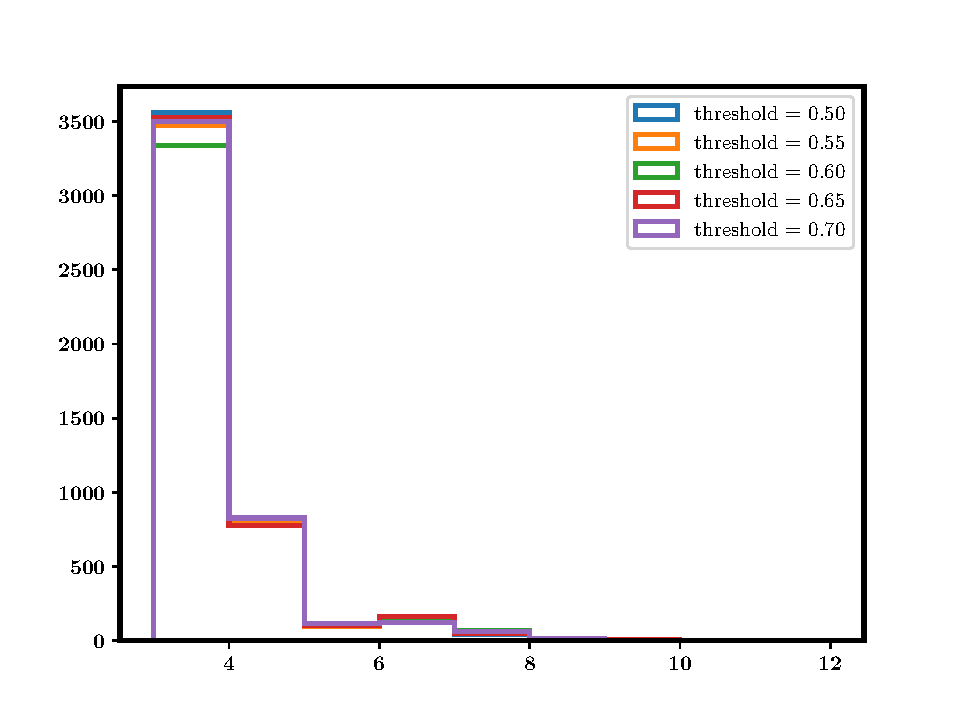
\includegraphics[scale=0.55]{histogram_of_Npoints}
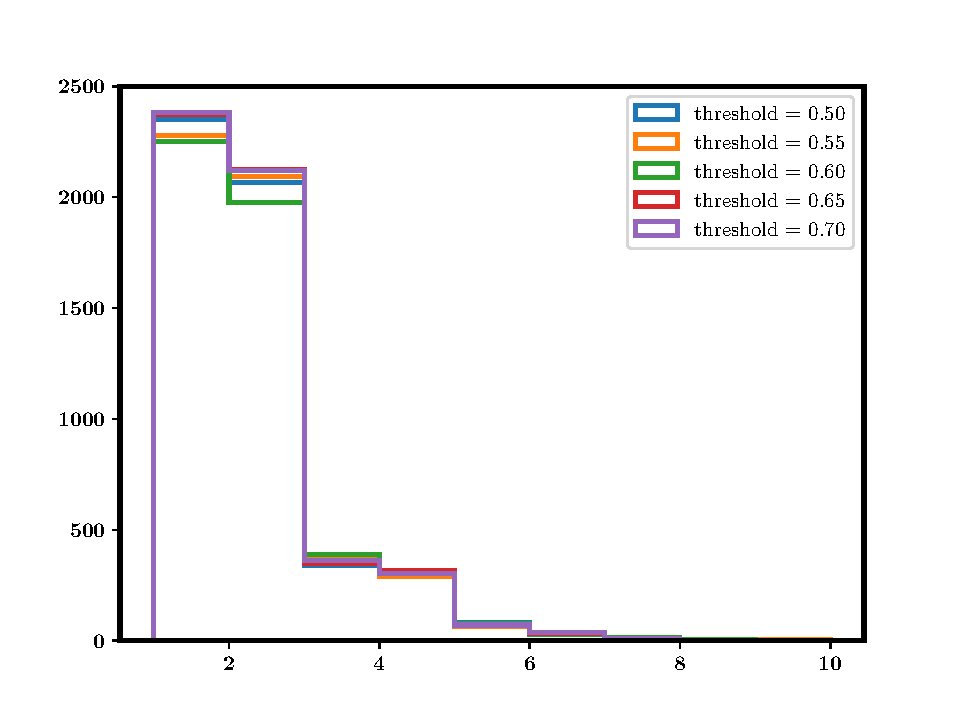
\includegraphics[scale=0.55]{histogram_of_Msum}
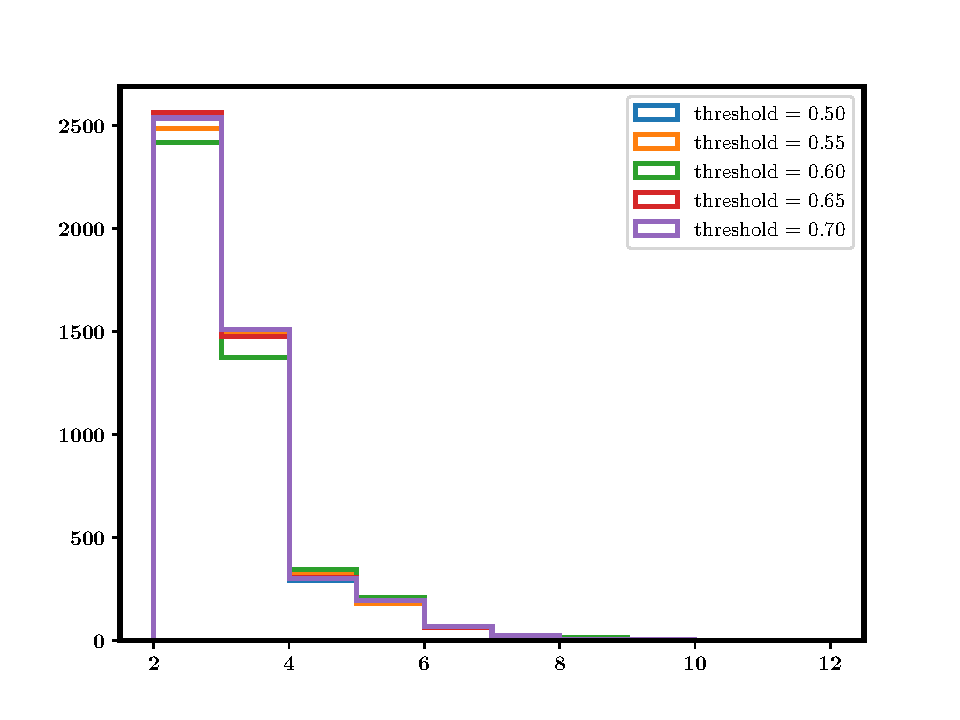
\includegraphics[scale=0.55]{histogram_of_Npairs}
\end{center}
\caption[Histograms of $\N$, $\M$ and $\Np$ with different values of $\thr$]{Histograms of $\N$ [top], $\M$ [middle] and $\Np$ [bottom] with different values of $\thr$. Since most of the pairs are non-identical, $\N$ is more likely to be even than odd, hence it shows regular dips at odd integers. It is observed that these parameters are insensitive to the value of $\thr$ chosen. Hence, it is fixed it at its most conservative upper limit throughout the work.
\label{fig:threshold_insensitiveness}}
\end{figure}


Next, we experiment the construction of $\al$ based on the three gross parameters, and flag random DPHs based on the different experimental values of these parameters. It turns out that both $\al = \M = 8$ and $\al = \Np = 8$ flag less than $1\%$ random DPHs, but this conclusion is seen to break down in the presence of bright GRBs like GRB160802A, since the number of photons in the DPH are  $\sim 10$ greater than the usual, resulting in random pixels getting paired and marked as hot pairs. Normalizing any of the parameters by the total number of photons does not help because extremely bright DPHstructures has total number of counts comparable to the total counts in random DPHs during GRBs, simply because the clustering illuminates its neighbourhood very brightly.




\begin{figure}
\begin{center}
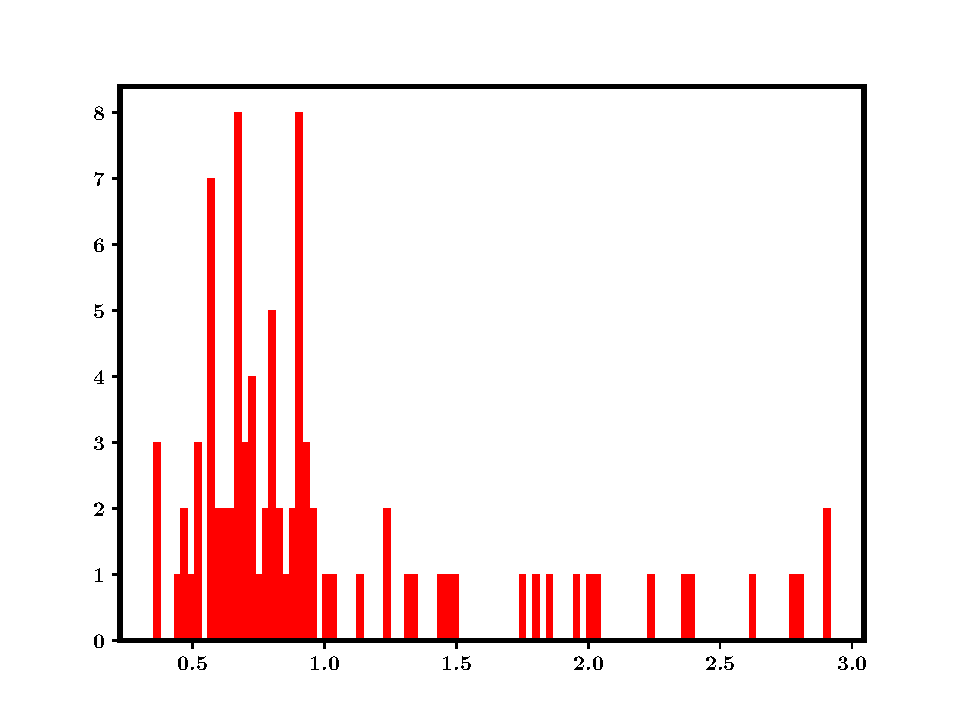
\includegraphics[scale=0.42]{GRB160802A--Q0--not_flagged}
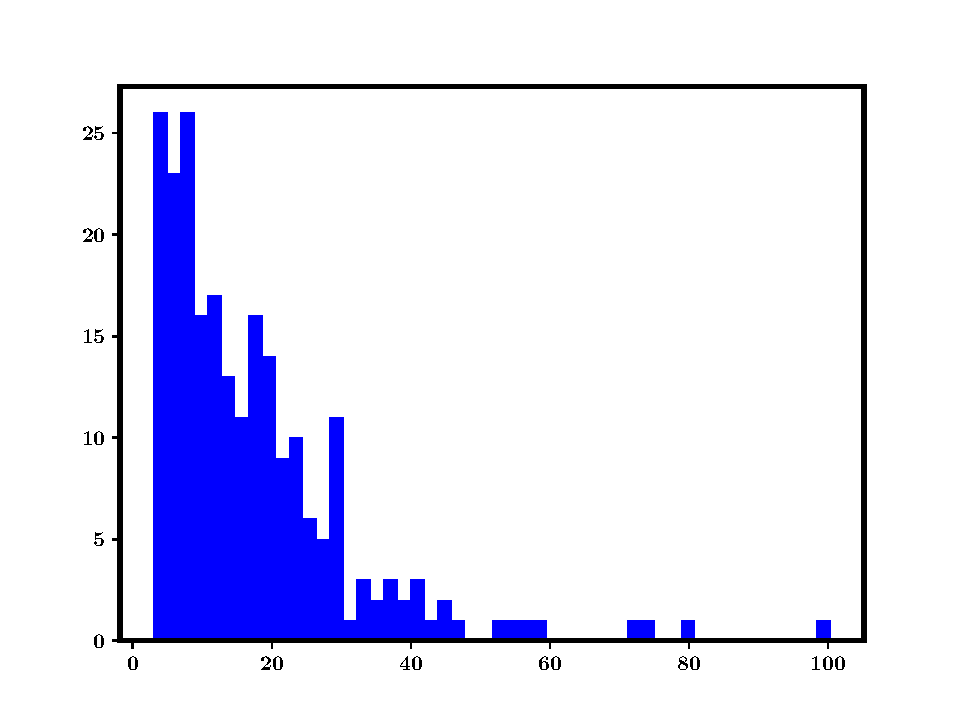
\includegraphics[scale=0.42]{GRB160802A--Q0--flagged}
\end{center}
\caption[Histograms of the parameter $\M / \N$]{\eL: Histogram of the parameter $\M / \N$ for the DPHs which are \emph{not} flagged. It does not reach $3$, the value of $\al$ used for flagging. \eR: Same for the ones that \emph{are} flagged. Although the total number of flagged DPHs in a typical dataset is much smaller than the number of DPHs that are flagged, most of them do not have any hot pairs, hence both $\M$ and $\N$ are zero, which are not plotted here, hence the numbers on the \eL\ appear smaller than those on the \eR. The sharp increase at values close to $4$ in \eR, compared to the rarity of those in \eL below $3$, demonstrates that the distinction is real. The reality of this distinction is also verified by manual examination of each DPH for long stretches of data, preferentially including weak as well as bright GRBs (examples in Figure \ref{fig:DPHs_flagged_and_unflagged}).
\label{fig:robustness_of_allowable=3}}
\end{figure}

\begin{figure}
\begin{center}
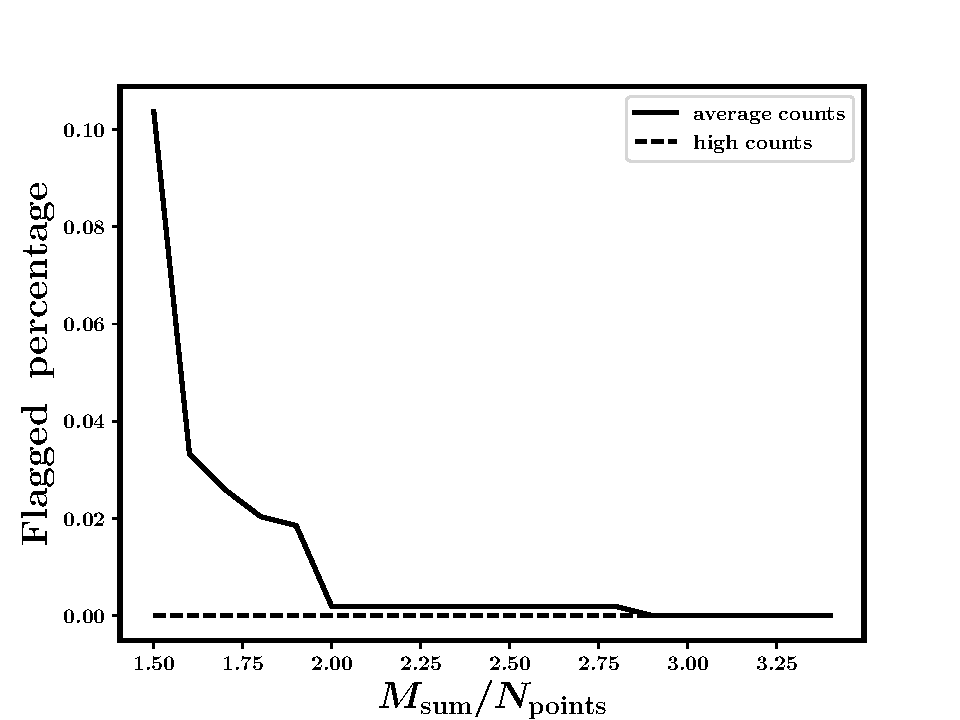
\includegraphics[scale=0.45]{DPH_simulations--flagged_percentage--zoom}
\end{center}
\caption[False alarm probability and the robustness of the algorithm]{Random DPHs are simulated with the event-rate as input. The parameter $\al$ is allowed to vary, and flagging is carried out on the random DPHs based on these variable values. The plot show the resulting number of DPHs flagged as a percentage of the total number of DPHs simulated [$54000$], as a function of the variable. Average count-rate of $150$ per second, and high count-rate during bright GRBs, $1500$ per second, are considered. The flagged percentage is $0$ for $ \M / \N > 3 $, proving the robustness of the algorithm for both the average data and during GRBs. In fact, it is more robust when the count-rate is \emph{more}, i.e. DPHs during bright GRBs have $\sim 0$ probability of getting flagged.
\label{fig:robustness_with_countrate}}
\end{figure}


To get around this, we define $\al = \M / \N $, because $\N$ normalizes for the additional $\M$ contribution from the pairs that are created due to chance co-incidence of a larger number of random events during GRBs. This simple modification fantastically tells clustered DPHs from random ones, see Figure \ref{fig:robustness_of_allowable=3}. The reason is that, although the total number of counts in a clustered DPH is large, the clustering is spread over only a few pixels, and the same pixels register many events. On the other hand, random DPHs with increased total counts, where the $\M$ is increased by co-incidental pairing of random events, have many such pairs which are themselves randomly distributed over the entire quadrant. It is also noted that in comparison to the above definition, $\al = \M / \Np$ does not do a better job because the small number of neighbouring pixels in a cluster tend to pair up with most of the other pixels in the cluster.

Random DPHs from GRBs and during average count-rates are examined along with DPHs that show clustering: it is seen that $\al = \M / \N = 3$ distinctly separates clustered DPHs from random ones, whether they are during a GRB or otherwise. This is verified first visually by looking at a significant number of DPHs by eye, and also demonstrated in Figs \ref{fig:robustness_of_allowable=3} and \ref{fig:robustness_with_countrate}. Examples of detected DPHstructures and also DPHs with non-detections are shown in Figure \ref{fig:DPHs_flagged_and_unflagged}.




\begin{figure}
\begin{center}
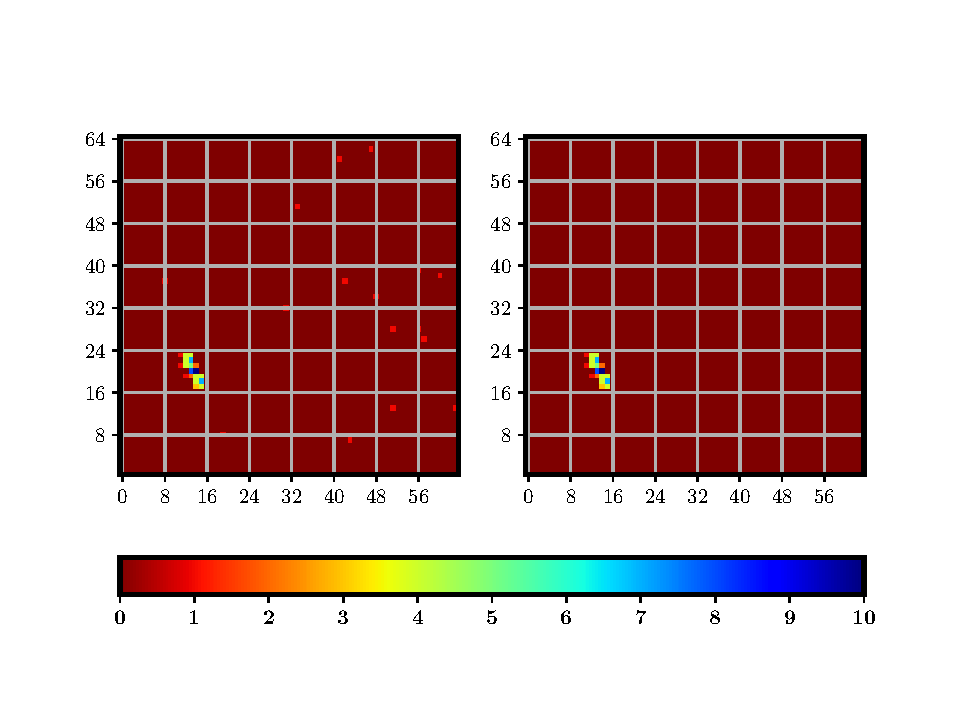
\includegraphics[scale=0.8]{Q0--peak_6262}
\end{center}
\begin{center}
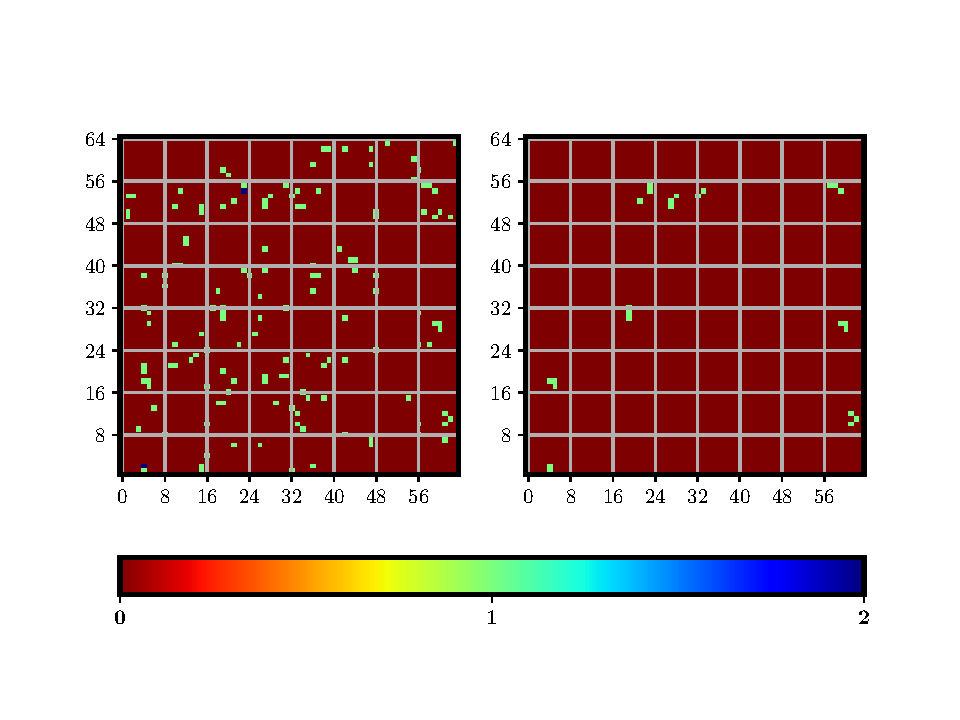
\includegraphics[scale=0.8]{Q0--peak_10009}
\end{center}
\caption[Examples of DPHs that are flagged, and those that are not]{\emph{Top}: On the \eL\ is a DPH which shows clustering [the colour-bar is of counts], with the identified clustered events shown in the \eR. \emph{Bottom}: On the \eL\ is a DPH that does not show clustering. The pairs that are used to test the clustering are explicitly shown in the \eR\ to demonstrate that the presence of such random pairs are not enough to flag this DPH.
\label{fig:DPHs_flagged_and_unflagged}}
\end{figure}
